\documentclass[8pt]{beamer}
\usepackage{tikz}
\usepackage[utf8]{vietnam}
\usepackage{amsmath}
\usepackage{graphicx}
\usepackage{wrapfig}
\usepackage{hyperref}
\usepackage{mathrsfs}
\usetheme{Copenhagen}
\usecolortheme{dolphin}
\setbeamertemplate{navigation symbols}{}
\setbeamertemplate{headline}{}
\title[Chương 1: Quy trình ADC/DAC] %optional
{Chương 1: Quy trình ADC/DAC}
\subtitle{Xử lý tín hiệu số}
\author[Xử lý tín hiệu số] % (optional)
{Tín Vũ}
\date[VLC 2021] % (optional)
{tinvu1309@gmail.com}
\begin{document}
\frame{\titlepage}
\begin{frame}{Mục lục}
\tableofcontents
\end{frame}
\begin{frame}{Giới thiệu playlist}
\section{Giới thiệu playlist}
	\begin{itemize}
		\item Mình là Tín Vũ, hiện đang là sinh viên học tại Trường Đại học Công nghệ, Đại học Quốc gia Hà Nội. Mình tạo playlist video này để hỗ trợ các bạn học môn \textbf{Xử lý tín hiệu số}.
\item Khác với môn học tiên quyết \alert{Tín hiệu hệ thống} trước đó, bài giảng môn học này \textbf{hoàn toàn bám sát với đề cương và giáo trình nội bộ} của trường mình, nên các bạn trường khác cần phải lưu ý rất kĩ điều này.
\item Không chỉ dừng lại ở lý thuyết, playlist này \textbf{có bổ sung hướng dẫn lập trình cơ bản bằng GNU Octave/Matlab} để vẽ phổ tín hiệu, đáp ứng tần số và thiết kế bộ lọc.
\item Môn học này bao gồm \textbf{6 chương}, các chương đều liên quan rất chặt chẽ với nhau nên hãy học cẩn thận ngay từ \alert{Chương 0} để ôn thi cuối kì đỡ vất vả.
	\end{itemize}
\end{frame}
\begin{frame}{Tài liệu tham khảo}
\section{Tài liệu tham khảo}
\begin{itemize}
		\item Tài liệu tham khảo chính: Giáo trình Xử lý tín hiệu số (Nguyễn Linh Trung, Trần Đức Tân, Huỳnh Hữu Tuệ, ĐHCN, 2012).
		\item Tài liệu tham khảo phụ: Discrete-time Signal Processing (Alan V.Oppenheim, 2nd edition). 
	\end{itemize}
\end{frame}
\begin{frame}{Quy trình xử lý tín hiệu số}
\section{Quy trình xử lý tín hiệu số}
\begin{figure}[h]
			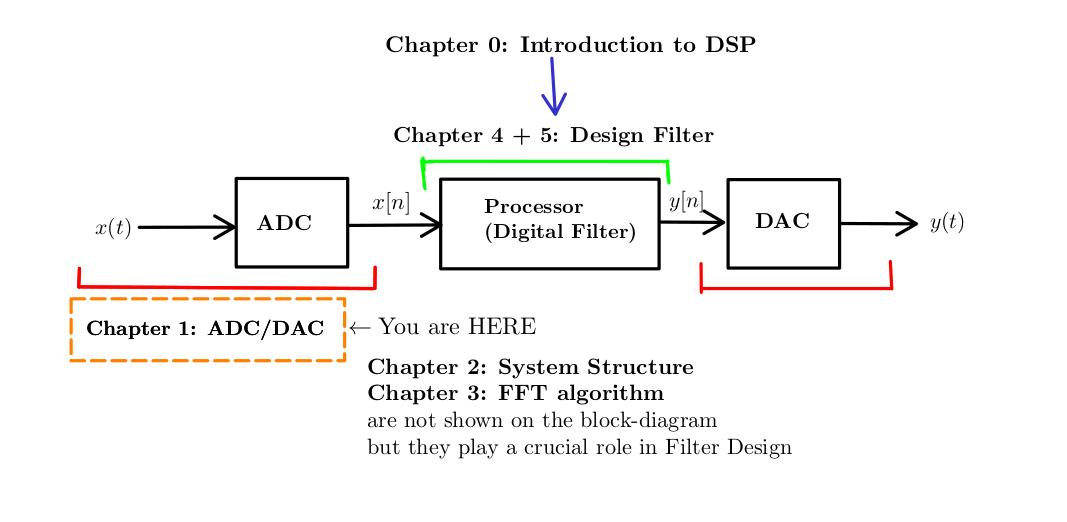
\includegraphics[width=1.1\textwidth]{1.jpg}
			\caption{DSP Learning Process}			\label{fig:re2}
		\end{figure}

\end{frame}
\begin{frame}{Quy trình ADC}
\section{Quy trình ADC}
\subsection{Quy trình lấy mẫu}
\begin{figure}[h]
			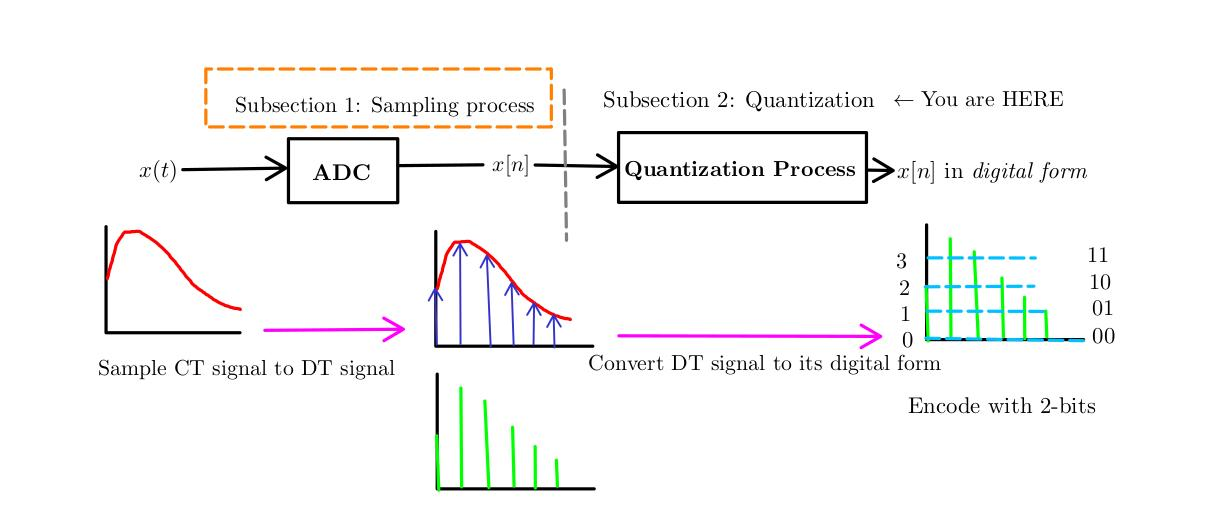
\includegraphics[width=1.1\textwidth]{2.jpg}
			\caption{ADC block diagram}			\label{fig:re3}
		\end{figure}


\end{frame}
\begin{frame}{Quy trình ADC}
\begin{itemize}
	\item Quy trình lấy mẫu
\end{itemize}
Trong môn học tiên quyết \alert{Tín hiệu và hệ thống} trước, ta đã đề cập định tính về quy trình lấy mẫu để chuyển đổi tín hiệu liên tục thành tín hiệu rời rạc. Bây giờ, ta muốn tìm một mối liên hệ rất chặt chẽ về mặt toán học giữa tín hiệu $x(t)$ và $x[n]$ trong \textbf{miền thời gian} và \textbf{miền tần số}, và từ kết quả này ta sẽ xây dựng phương pháp chuyển đổi ngược tín hiệu rời rạc thành tín hiệu liên tục.
\begin{figure}[h]
			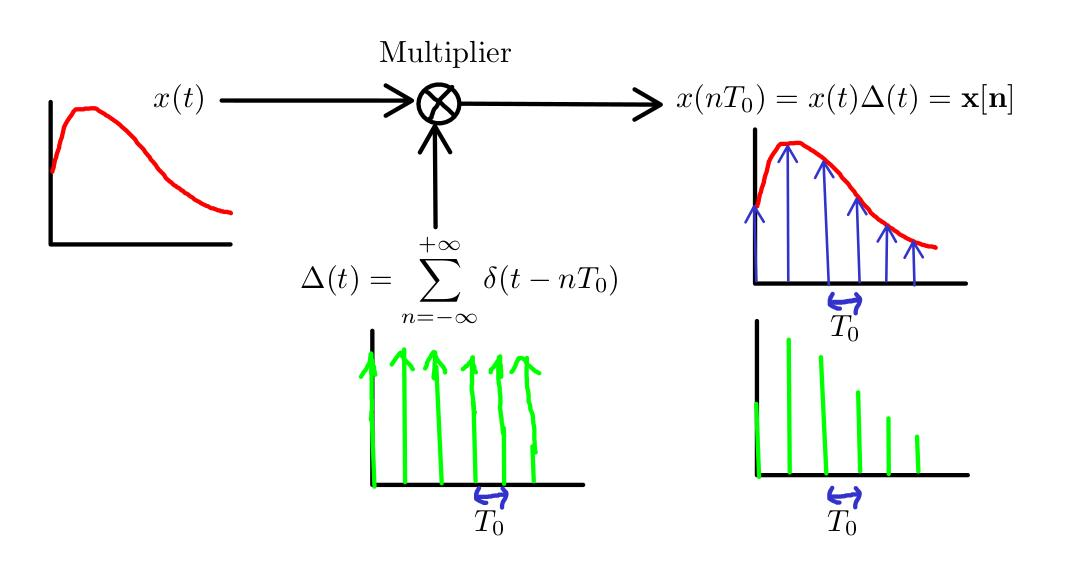
\includegraphics[width=0.8\textwidth]{3.jpg}
			\caption{Sampling process}			\label{fig:re4}
		\end{figure}

\end{frame}
\begin{frame}{Quy trình ADC}
	Trong môn học Xử lý tín hiệu số (từ giờ ta sẽ gọi tắt là DSP - Digital Signal Processing), các kí hiệu tần số \alert{ngược với môn Tín hiệu và hệ thống}, ta quy ước kí hiệu $\Omega$ cho tần số \textbf{liên tục} và $\omega$ cho tần số \textbf{rời rạc}. Từ mối liên hệ giữa $x(t)$ và $x[n]$, ta có:
\begin{equation*}
\begin{split}
	x[n]=x(nT_{0})=x(t)\Delta(t)=x(t)\sum_{n=-\infty}^{+\infty}\delta(t-nT_{0})
\end{split}
\end{equation*}
Dễ dàng nhận thấy $\Delta(t)$ có dạng \textbf{chuỗi Fourier liên tục (CTFS)}, ta thử tìm cách biểu diễn tín hiệu này về dạng chuỗi CTFS để phân tích trong miền tần số như sau:
$$\Delta(t)=\sum_{n=-\infty}^{+\infty}c_{n}e^{jn\Omega_{0}t}$$
$$c_{n}=\frac{1}{T_{0}}\int_{T_{0}}\Delta(t)e^{-jn\Omega_{0}t}dt=\frac{1}{T_{0}}\int_{-\frac{T_{0}}{2}}^{+\frac{T_{0}}{2}}\left[\sum_{n=-\infty}^{+\infty}\delta(t-nT_{0})\right]e^{-jn\Omega_{0}t}dt=\frac{1}{T_{0}}$$
Vậy ta thu được chuỗi CTFS của tín hiệu $\Delta(t)$: 
$$\Delta(t)=\frac{1}{T_{0}}\sum_{n=-\infty}^{+\infty}e^{jn\Omega_{0}t}$$
Ta xét biến đổi Fourier liên tục (CTFT) và tính chất \textbf{dịch trong miền tần số}:
\end{frame}
\begin{frame}{Quy trình ADC}
\begin{equation*}
\begin{split}
	X(\omega)=\mathscr{F}(x(t)\Delta(t))=\frac{1}{T_{0}}\mathscr{F}\left(x(t)\sum_{n=-\infty}^{+\infty}e^{jn\Omega_{0}t}\right)=\frac{1}{T_{0}}\sum_{n=-\infty}^{+\infty}X(\Omega-n\Omega_{0})
\end{split}
\end{equation*}
Ta phác họa đáp ứng biên độ của tín hiệu liên tục và rời rạc tương ứng, gọi $\Omega_{M}$ là tần số biên (tức thành phần tần số lớn nhất trong phổ của tín hiệu liên tục):
\begin{figure}[h]
			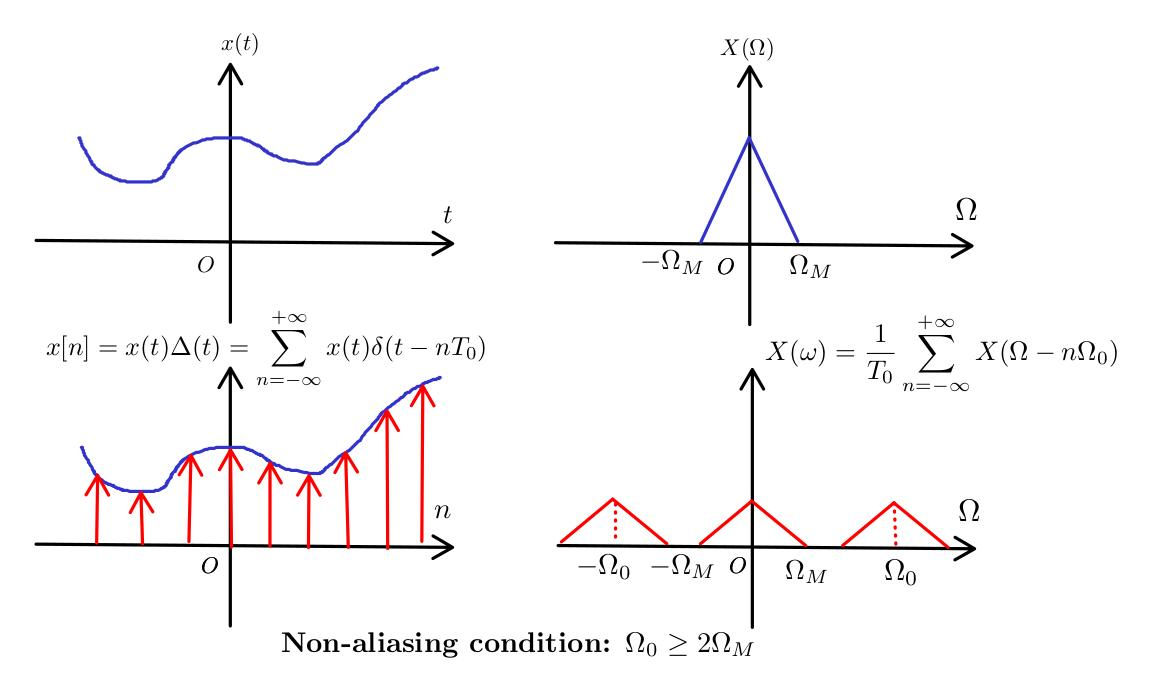
\includegraphics[width=0.8\textwidth]{4.jpg}
			\caption{CT and FT signal spectrum}			\label{fig:re5}
		\end{figure}

\end{frame}
\begin{frame}{Quy trình ADC}
	Để phổ của tín hiệu rời rạc không bị gập (aliasing or folding), từ hình vẽ ta hiển nhiên thấy: $$\Omega_{0}\geq2\Omega_{M}\Leftrightarrow f_{0}\geq 2f_{M}$$
	Chúng ta gọi hằng số: $$f_{N}=2f_{M}$$  là \alert{tốc độ Nyquist} của tín hiệu $x(t)$. Vậy để phổ của tín hiệu rời rạc không bị chồng lấn (overlap) thì ta phải \textbf{lấy mẫu tín hiệu $x(t)$ với \alert{tốc độ} tối thiểu bằng hai lần thành phần tần số cao nhất trong tín hiệu liên tục}.
	\\ Hiển nhiên từ công thức: $$x[n]=x(nT_{0})$$ với cặp $\omega-\Omega$ là thành phần tần số tương ứng giữa tín hiệu rời rạc và tín hiệu liên tục, ta dễ dàng suy ra mối liên hệ: $$\omega=\Omega T_{0}$$
	Kết quả trên hoàn toàn khớp với phân tích định tính ta đã thực hiện trong môn học \alert{Tín hiệu và hệ thống} trước, phổ của tín hiệu rời rạc \textbf{luôn tuần hoàn}.
\end{frame}
\begin{frame}{Quy trình ADC}
	\subsection{Quy trình lượng tử hóa}
\begin{itemize}
	\item Quy trình lượng tử hóa
\end{itemize}
\begin{figure}[h]
			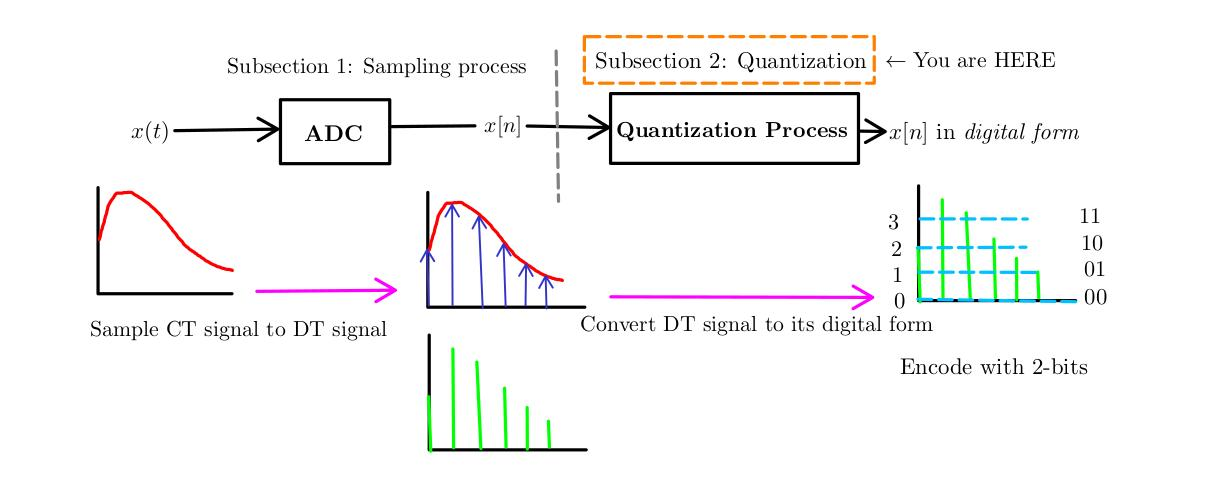
\includegraphics[width=0.8\textwidth]{5.jpg}
			\caption{Quantization Process}			\label{fig:re6}
		\end{figure}
		Sau khi đã rời rạc hóa tín hiệu liên tục, ta muốn "định mức" chúng vào các mức lượng tử để mã hóa thành các số nhị phân tương ứng (do hệ thống máy tính số làm việc với các bit nhị phân). Quy trình này được gọi là \alert{lượng tử hóa}, từ hình minh họa dưới đây, ta định nghĩa các khái niệm:
		\begin{itemize}
			\item Mức lượng tử $\Delta$: $$\Delta=\frac{V_{max}-V_{min}}{2^{n}}$$
			\item Số bit lượng tử $n$.
		\end{itemize}
\end{frame}
\begin{frame}{Quy trình ADC}
\begin{figure}[h]
			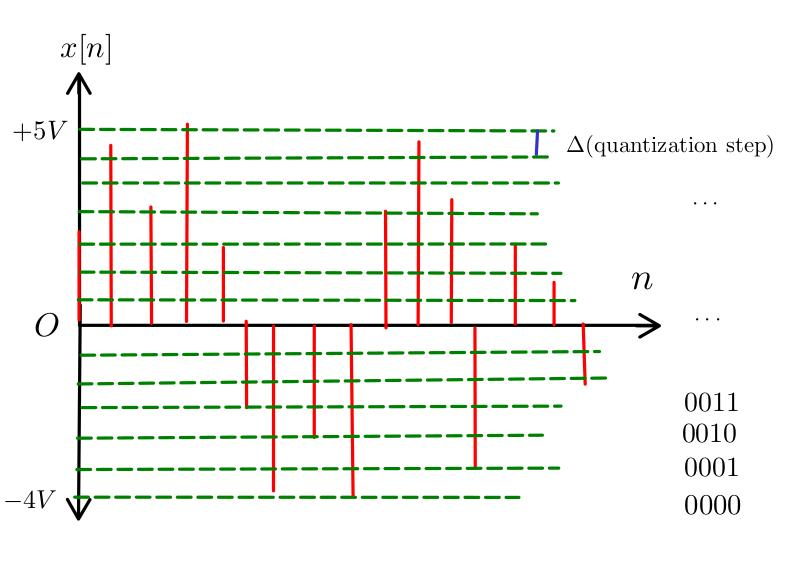
\includegraphics[width=0.8\textwidth]{6.jpg}
			\caption{Using 4 bits to quantizate DT signal}			\label{fig:re7}
		\end{figure}
\end{frame}
\begin{frame}{Quy trình ADC}
	Ví dụ: tín hiệu $x(t)=2\cos{(500\pi t)}$ được lấy mẫu với \alert{tốc độ} $f_{sam}=3\text{k (sample/s)}$, sau đó được lượng tử hóa với độ phân giải $8$ bit. 
	\\ Dễ thấy $f_{N}=2f_{M}=500\text{Hz}$, và $f_{sam}>f_{N}$ nên \textbf{hiện tượng gập phổ không xảy ra}. Tín hiệu rời rạc được xác định qua phương trình:
	$$x[n]=x(nT_{sam})=x\left(\frac{n}{f_{sam}}\right)=2\cos\left(\frac{\pi n}{6}\right)$$
Hiển nhiên $-2\leq x[n]\leq +2$, nên áp dụng công thức tìm mức lượng tử $\Delta$ ta thu được:
$$\Delta=\frac{V_{max}-V_{min}}{2^{n}}=\frac{2-(-2)}{2^{8}}=\frac{1}{64}$$
Nếu ta lấy mẫu với \alert{tốc độ} $f_{sam}=400$ (sample/s), phổ của tín hiệu rời rạc sẽ bị ảnh hưởng như thế nào? Hiển nhiên ta thấy khi lấy mẫu ở tốc độ thấp \textbf{hiện tượng gập phổ có xảy ra}.
\begin{figure}[h]
			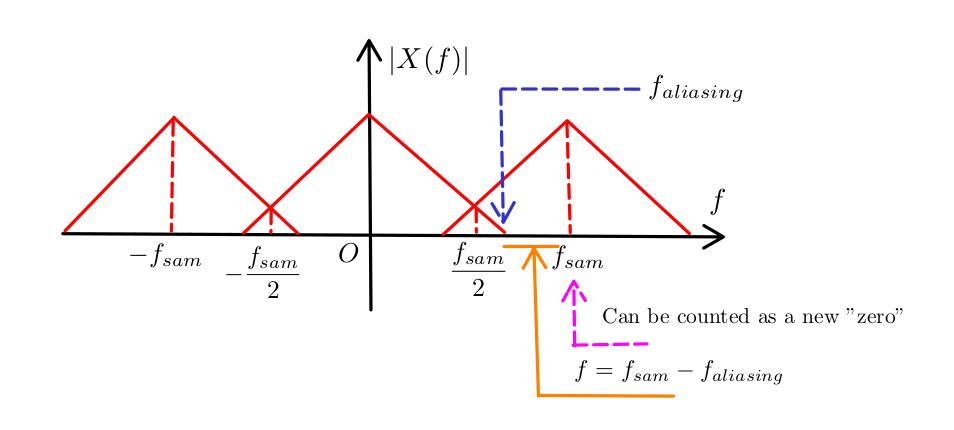
\includegraphics[width=0.6\textwidth]{9.jpg}
			\caption{Aliasing Phenomenon}			\label{fig:re8}
		\end{figure}
\end{frame}
\begin{frame}{Quy trình ADC}
	Từ công thức: $$0<\pm f_{aliasing}+k f_{sam}<\frac{f_{sam}}{2}$$ 
	và công thức tìm tín hiệu sau khi lấy mẫu: $$x[n]=x\left(\frac{nf}{f_{sam}}\right)$$
Ta dễ dàng xác định được tần số của tín hiệu sau khi bị gập phổ, và tín hiệu rời rạc tương ứng thu được là:
$$x[n]=x\left(\frac{nf}{f_{sam}}\right)=2\cos\left(\frac{3\pi n}{8}\right)$$
Ta có thể tăng độ phân giải từ $8$ bit lên $16$ hoặc $32$ bit để tín hiệu rời rạc thu được dưới dạng mã nhị phân chính xác hơn. Nói chung, độ phân giải càng cao thì tín hiệu rời rạc càng chính xác. 
\end{frame}
\begin{frame}{Quy trình DAC}
	\section{Quy trình DAC}
\begin{figure}[h]
			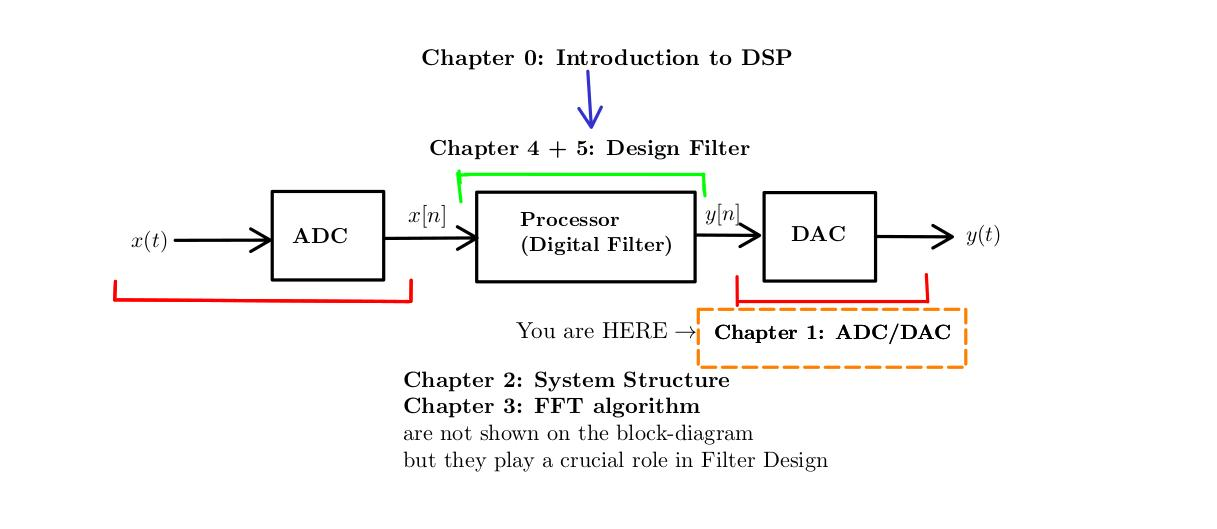
\includegraphics[width=1.1\textwidth]{7.jpg}
			\caption{DSP Learning process}			\label{fig:re8}
		\end{figure}

\end{frame}
\begin{frame}{Quy trình DAC}
	Từ phổ tần số của cặp tín hiệu $x(t)$ và $x[n]$ đã được vẽ ở phần trước; ta dễ dàng thấy rằng để khôi phục được \textbf{phổ} tín hiệu $x(t)$ hoàn chỉnh từ $x[n]$, ta cần thiết kế một \textbf{bộ lọc thông thấp} (Low-pass filter) với điều kiện tần số cắt (cut-off frequency) như sau (ta tạm thời bỏ qua yếu tố khôi phục độ lớn bằng bộ khuếch đại do hao hụt bởi hằng số, mà chỉ quan tâm đến khôi phục phổ):
\begin{figure}[h]
			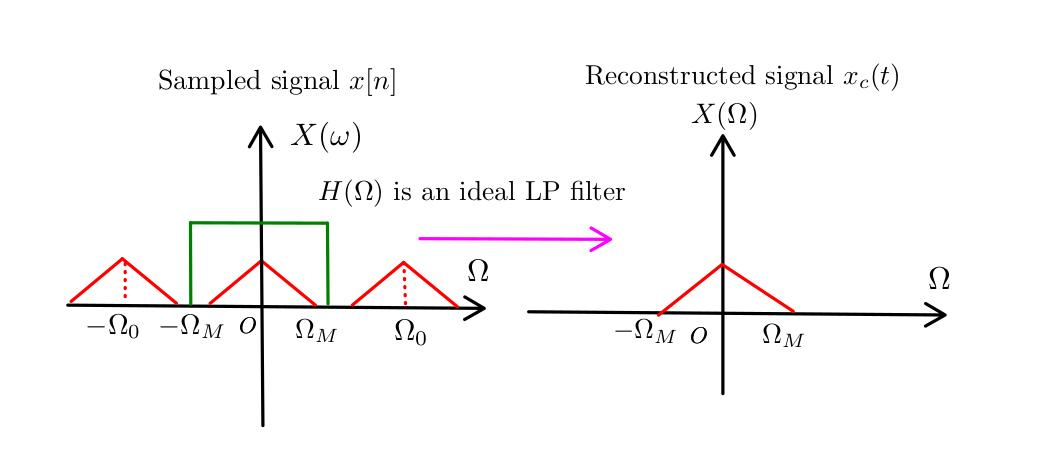
\includegraphics[width=1.1\textwidth]{8.jpg}
			\caption{Reconstruct CT signal spectrum}			\label{fig:re9}
		\end{figure}


\end{frame}
\begin{frame}{Quy trình DAC}
Với đáp ứng biên độ của bộ lọc thông thấp $H(\Omega)$:
\begin{equation*}
H(\Omega)=
\begin{cases}
	1\quad(|\Omega|\leq\frac{\Omega_{0}}{2})\\
	0\quad(\text{otherwise})\\
\end{cases}
\end{equation*}
\\ Ta chọn tần số cắt của bộ lọc $$\Omega_{C}=\frac{\Omega_{0}}{2}$$
Dễ thấy \textbf{thành phần tần số lớn nhất} mà bộ lọc thông thấp có thể khôi phục được hoàn hảo từ tín hiệu rời rạc là: $$\Omega_{M}\leq\frac{\Omega_{0}}{2}\Leftrightarrow f_{M}\leq\frac{f_{0}}{2}$$
Ta gọi hằng số $f_{N}=\frac{f_{0}}{2}$ là \alert{tần số Nyquist của tín hiệu}, là thành phần tần số \textbf{lớn nhất} của tín hiệu tương tự $x(t)$ có thể khôi phục lại được bằng bộ lọc thông thấp trong khối DAC có \textbf{độ lớn bằng một nửa tần số lấy mẫu}.
\\  Ta phải phân biệt rất rạch ròi giữa hai khái niệm \alert{tốc độ Nyquist} và \alert{tần số Nyquist}, chúng có kí hiệu giống nhau nhưng \textbf{thứ nguyên và ý nghĩa vật lý hoàn toàn khác nhau}, cũng như hai mặt sấp-ngửa của một đồng xu vậy.

\end{frame}
\begin{frame}{Quy trình DAC}
Sau khi đã thấy mối quan hệ giữa $x[n]$ và $x_{c}(t)$ trong miền tần số, ta muốn tìm mối quan hệ của chúng tương ứng trong miền thời gian; và so sánh sự sai khác giữa tín hiệu $x_{c}(t)$ với tín hiệu $x(t)$.
Ta có:
$$\mathscr{F}^{-1}[X_{c}(\Omega)]=\mathscr{F}^{-1}[X(\omega)H(\Omega)]\Rightarrow x_{c}(t)=x(nT_{0})*h(t)$$
Có nhiều cách để tìm đáp ứng xung $h(t)$, các bạn có thể tìm gián tiếp bằng tính chất đối ngẫu (duality) của CTFT, nhưng ở đây mình sẽ tìm trực tiếp bằng công thức ICTFT:
\begin{equation*}
\begin{split}
	h(t)&=\frac{1}{2\pi}\int_{-\infty}^{+\infty}H(\Omega)e^{j\Omega t}d\Omega=\frac{1}{2\pi}\int_{-\frac{\Omega_{0}}{2}}^{+\frac{\Omega_{0}}{2}}e^{j\Omega t}d\Omega=\frac{\sin\left(\frac{\Omega_{0}t}{2}\right)}{\pi t}=\frac{\sin\left(\frac{\pi t}{T_{0}}\right)}{\pi t}\\
		 &= \alert{T_{0}\text{sinc}\left(\frac{t}{T_{0}}\right)}
\end{split}
\end{equation*}
với hàm sinc được định nghĩa: $$\text{sinc}(x)=\frac{\sin(\pi x)}{\pi x}$$ 
\end{frame}
\begin{frame}{Quy trình DAC}
Vậy hiển nhiên ta có:
\begin{equation*}
\begin{split}
	x_{c}(t)&=x(nT_{0})*h(t)=\left[\sum_{n=-\infty}^{+\infty}x(t)\delta(t-nT_{0})\right]*T_{0}\text{sinc}\left(\frac{t}{T_{0}}\right)\\ &=\alert{T_{0}\sum_{n=-\infty}^{+\infty}x(t)\text{sinc}\left(\frac{t-nT_{0}}{T_{0}}\right)}
\end{split}
\end{equation*}
Đây chính là phương trình của tín hiệu liên tục $x_{c}(t)$ có thể khôi phục được từ khối DAC.
Công thức này còn được gọi là \textbf{công thức nội suy của tín hiệu $x(t)$}.
\end{frame}
\end{document}
